% -----------------------------------------------------------------------------
%   Arquivo: ./02-elementos-textuais/resultados.tex
% -----------------------------------------------------------------------------



\chapter{Análise e Discussão dos Resultados}

Como era de se esperar, o algoritmo MaxMin1 apresentou uma complexidade de 2(n-1), onde n é o tamanho do vetor, no caso, 10.000. Portanto, como ilustrado no gráfico abaixo, temos uma linha reta. Já para o algoritmo MaxMin2, percebemos uma performance melhor, uma vez que não temos a "comparação" de todos os elementos do vetor para encontrar o Maior e Menor valor. 

Segue a ilustração abaixo. 

\begin{figure}[!htb]
	\centering
	\caption{MaxMin1 x MaxMin2}
	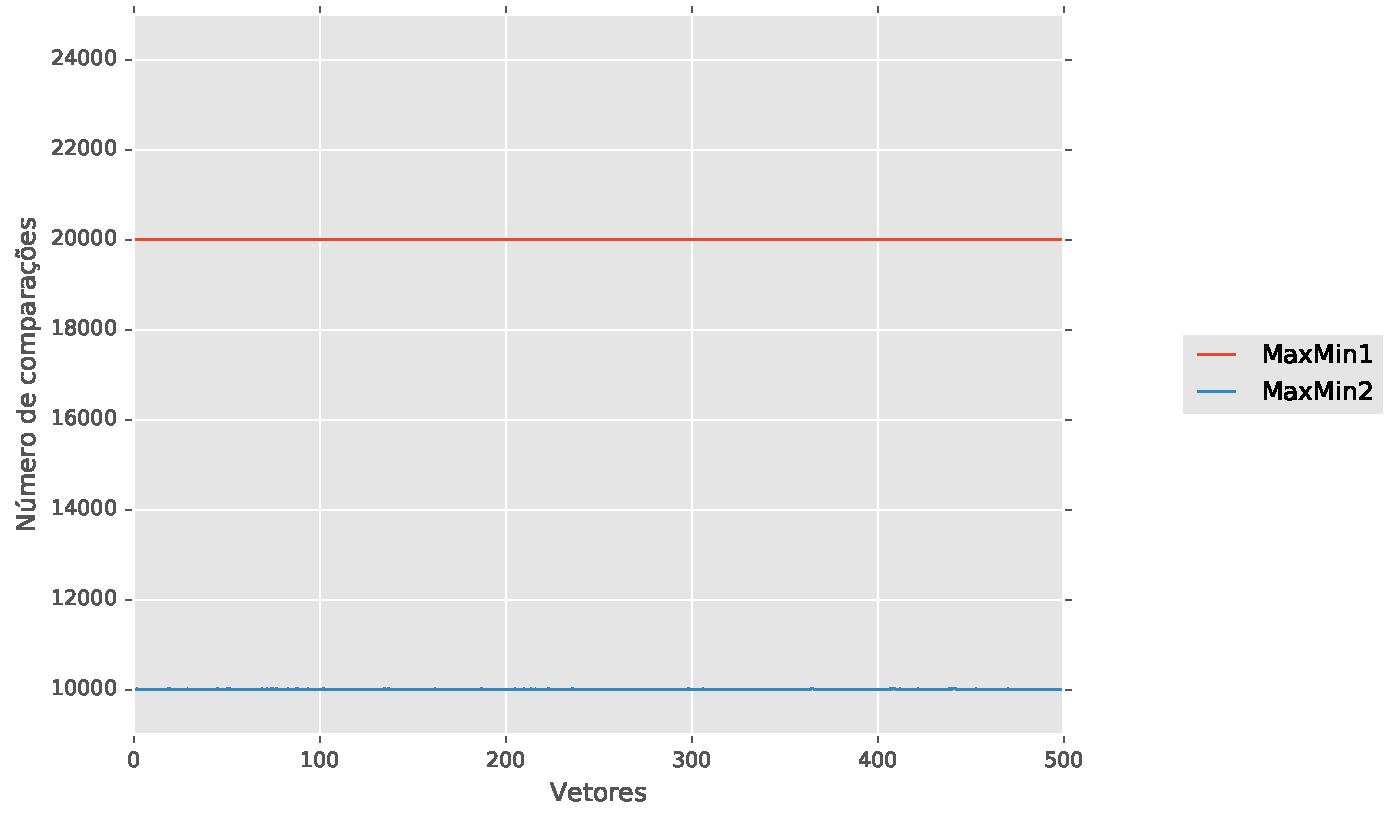
\includegraphics[width=0.8\textwidth]{./04-figuras/MaxMin1xMaxMin2.pdf}
	\fonte{Própria}
	\label{fig:maxmin1vsmaxmin2}
\end{figure}

\pagebreak
Apesar de não visivel (devido a escala do gráfico), o método MaxMin2 apresentou uma pequena variação de seus contadores. Esta pequena variação pode ser visualizada no gráfico abaixo onde a escala foi mudada. 


\begin{figure}[!htb]
	\centering
	\caption{MaxMin2}
	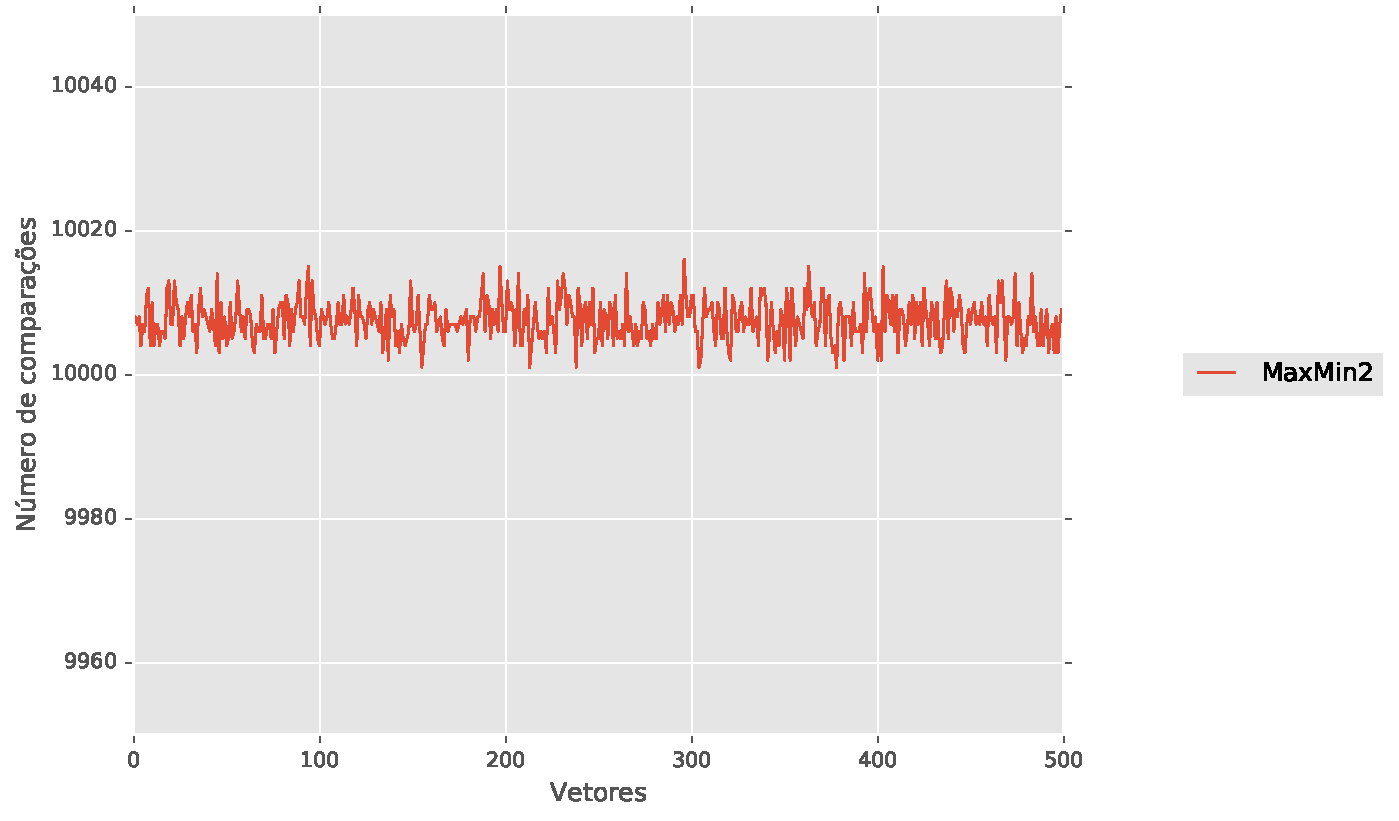
\includegraphics[width=0.8\textwidth]{./04-figuras/MaxMin2.pdf}
	\fonte{Própria}
	\label{fig:maxmin2}
\end{figure}



O valor médio encontrado pelo algoritmo MaxMin1 e MaxMin2 estão ilustrados na tabela a seguir: 

\begin{table}[!htb]
	\centering
	\caption[Médias encontradas]{Médias encontradas.
	\label{tab:medias}}
	\begin{tabular}{rrrrr}
		\toprule
			& Média &  \\
		\midrule
			MaxMin1 & 19998.00 \\
			MaxMin2 & 10007.74 \\
		\bottomrule
	\end{tabular}
\end{table}


